\documentclass{article}

\usepackage[version=3]{mhchem} % Package for chemical equation typesetting
\usepackage{siunitx} % Provides the \SI{}{} and \si{} command for typesetting SI units
\usepackage{graphicx} % Required for the inclusion of images
\usepackage{natbib} % Required to change bibliography style to APA
\usepackage{amsmath} % Required for some math elements 

\setlength\parindent{0pt} % Removes all indentation from paragraphs

\renewcommand{\labelenumi}{\alph{enumi}.} % Make numbering in the enumerate environment by letter rather than number (e.g. section 6)

%\usepackage{times} % Uncomment to use the Times New Roman font
\usepackage{hyperref}
\usepackage{listings}


%----------------------------------------------------------------------------------------
%	DOCUMENT INFORMATION
%----------------------------------------------------------------------------------------
\title{Programming of Supercomputers \\ Final Report} % Title
\author{Denys \textsc{Sobchyshak} and Denys \textsc{Korzh}} % Author name
\date{\today} % Date for the report

\begin{document}
\maketitle

%----------------------------------------------------------------------------------------
%	SECTION 1
%----------------------------------------------------------------------------------------
\section{Introduction}
Programming of Supercomputers lab course deals to a great extent with a code that simulates 
flow and heat transfer within arbitrary complex geometries with fixed boundaries, also known 
as an AVL FIRE\textregistered\ benchmark. Most of the effort was focused on parallelizing and 
optimizing the benchmark code in order to prepare it for execution in multiprocessor environments.
During the semester we had to complete the following tasks:
\begin{itemize}
	\item single-core optimization
	\item analysis of I/O behavior
	\item visualization
	\item 3-steps MPI parallelization
	\item performance tuning
\end{itemize}
In this report we will take a brief look at the summary of single-core optimization results 
and then move forward to parallelization aspects and their respective in depth analysis. 
It is important to note that all the measurements were carried out on a SuperMUC thin node.
 
%----------------------------------------------------------------------------------------
%	SECTION 2
%----------------------------------------------------------------------------------------
\section{Single-core optimization}
Quite often the great speedup potential of single-core execution of applications is overseen by
many developers and instead all the effort is put into the parallelization step. This leads to
inefficient usage of resources and poor scalability.
\\\\
This part of the course was focused solely on sequential optimization as a result of which 
we wanted to see how different optimization techniques relate to each other and what potential 
benefits our simulation code might obtain from them.
\\\\
The solver's execution was split into 3 main phases: input, computation and output. Analysis 
included collecting the following key characteristics for the computation phase using 2 input 
files (tjunc, cojack) and several optimization levels (-O1, -O2, -O3):
\begin{itemize}
	\item execution time
	\item Mflops
	\item L2 cache miss rate
	\item L3 cache miss rate
\end{itemize}
In addition we analysed the effect of vectorization on the computation phase using various
compiler flags (-[no]-vec, -vec-report, -xhost).

\subsection{Performance measurements using PAPI}
In order to collect the measurements following hardware measurement counters of the
Performance Application Programming Interface (PAPI) were used:\\
\begin{center}
\begin{tabular}{l|c}
	\hline
	Event & Description \\
	\hline
	PAPI\_DP\_OPS & Floating point operations; optimized to count vector operations \\
	PAPI\_L2\_TCM & Level 2 cache misses \\
	PAPI\_L2\_TCA & Level 2 total cache accesses \\
	PAPI\_L3\_TCM & Level 3 cache misses \\
	PAPI\_L3\_TCA & Level 3 total cache accesses \\
\end{tabular}
\end{center}
and consequently the next formulas to compute metrics were used:
\begin{center}
	$MFLOPS=\frac{PAPI\_FP\_OPS}{end\_time\_usec - start\_time\_usec}$
\end{center}
\begin{center}
	$L2\_CACHE\_MISS\_RATE=\frac{PAPI\_L2\_TCM}{PAPI\_L2\_TCA}*100$
\end{center}
\begin{center}
	$L3\_CACHE\_MISS\_RATE=\frac{PAPI\_L3\_TCM}{PAPI\_L3\_TCA}*100$
\end{center}
where end\_time\_usec and start\_time\_usec are corresponding PAPI start and end time values.

\subsubsection{Execution time}
With regard to execution time we observed that runtime of the computation phase decreased by roughly 23\% once the -O3 flag was utilized. Such agressive loop optimization for speed can be seen on figure \ref{fig:1}.
\begin{figure}[h!]
	\begin{center}
		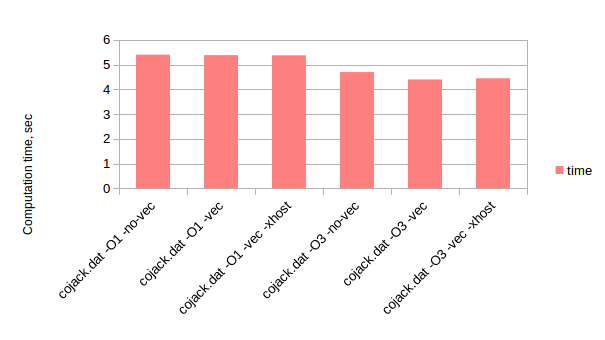
\includegraphics[width=0.8\textwidth]{comp-time}
		\caption{Comparison of computational time}
		\label{fig:1}
	\end{center}
\end{figure}

\subsubsection{Cache miss rates}
Using -03 flag increased the cache miss rates for both L2 and L3 caches by a rough 22\%. Such effects of vecotorisation on cache miss rates can be seen on figure \ref{fig:2}.
\begin{figure}[h!]
	\begin{center}
		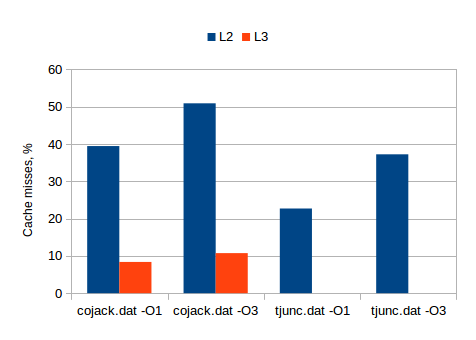
\includegraphics[width=0.8\textwidth]{cache-misses}
		\caption{Comparison of cache misses}
		\label{fig:2}
	\end{center}
\end{figure}

\subsubsection{MFLOPS counters}
We observed that once -O3 flag was employed measured MLUPS increased only marginally, aAnalysis of such a delicate matter is hard to perform with raw instruments, however it is known that optimization might include various techniques like excluding common calculations out of loops, pre-calculating expressions, fusing constants and so on which will decrease the number of operations performed while the actual runtime might not decrease substantially.

\subsubsection{Effect of vectorization}
While carrying out measurements of vectorized versus novectorised banchmark runtime under different optimization options we have observed that enabled vectorization versus diabled one decreases the runtime of simulation by roughly 7\%. Furthermore, we measured computation time while having -xhost flag enabled and it slows down the simulation by around 1.2\%. This is most likely observed because vectorization can sometimes slow execution due to pipeline synchronization, data movement timing or other issues.

%----------------------------------------------------------------------------------------
%	SECTION 3
%----------------------------------------------------------------------------------------
\section{I/O performance analysis}
Manipulating data files is very slow compared to accessing the main memory. This can be considerably improved by using a more concise data format such as binary. After comparing input file sizes and the time it takes to load them we have noticed a drastic fall in both processing time and binary file sizes. Visualized comparison of loading times and file sizes is shown on figure \ref{fig:3}.

\begin{figure}[h!]
\begin{center}
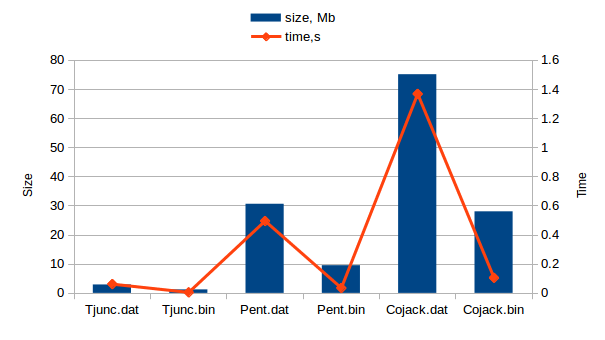
\includegraphics[width=0.8\textwidth]{time-size}
\caption{Comparison of file sizes and their read times}
\label{fig:3}
\end{center}
\end{figure}
%----------------------------------------------------------------------------------------
\end{document}